%!TEX root = ../index.tex
Da die Wahl des zu verwendenden Protokolls auf OpenID fällt, wird an dieser Stelle die Funktionsweise von OpenID erklährt. Es ist nicht Bestandteil dieser Arbeit das OpenID Protokoll in Python zu implementieren, da dazu bereits eine Library existiert welche auch gewartet wird. Ryan Boyd von Google empfielt in einem Talk ausdrücklich davon abzusehen openid selber zu implementieren \cite[0:16:08]{googleioopenid}.

\section{Übersicht}
\label{sec:übersicht}
OpenID wurde entwickelt damit sich Benutzer an fremden Webseiten anmelden können, ohne dass sie ein neues Passwort kreieren müssen. OpenID ermöglicht es Benutzern eines \glsdisp{OpenID-Provider}{OpenID-Providers} sich an Webseiten welche als \gls{OpenID-Relying-Party} fungieren anzumelden. 

\section{Ablauf}
\label{sec:ablauf}
Abbildung~\ref{fig:openid_ablauf} zeigt den Ablauf der Authentisierung über OpenID. Es handelt sich hier um den einfachsten Ablauf. Es gibt noch weitere Abläufe in denen zum Beispiel der Provider und die Relying-Party ein Shared Secret mittels Diffie Hellman\cite{rfc2631} vereinbaren um damit die OpenID-Response mit einem HMAC\cite{rfc2104} zu versehen. Damit sind die Schritte 9 und 10 nicht mehr nötig, da nach dem Schritt 8 die Relying-Party bereits sicherstellen kann, dass die Response nicht verändert wurde und vom Provider stammt.
\begin{figure}[H]
  \centering
	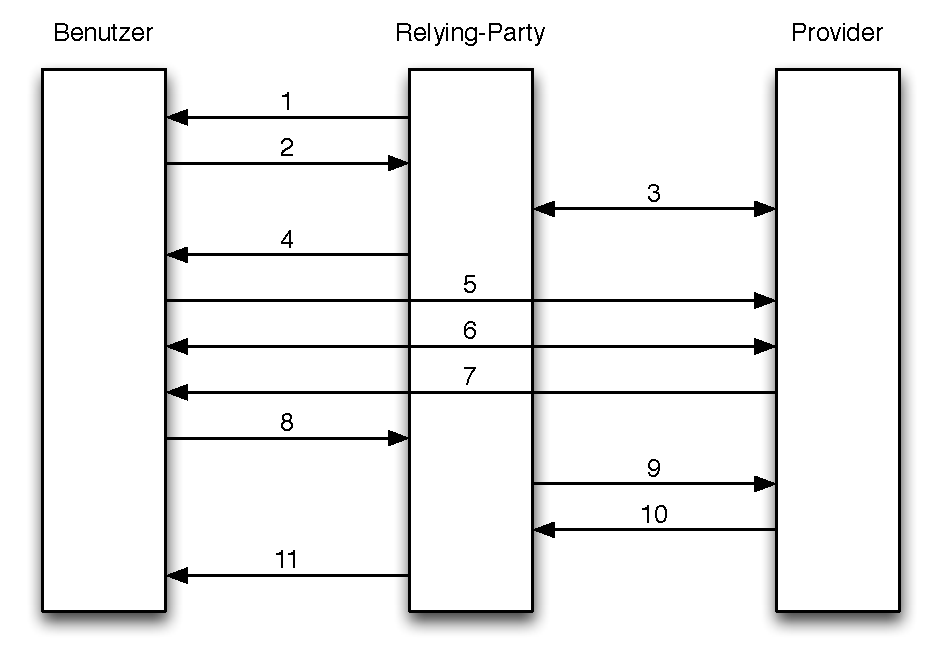
\includegraphics[width=0.70\textwidth]{include/openid1.pdf}
	\caption{OpenID Ablauf}
	\label{fig:openid_ablauf}
\end{figure}

\begin{enumerate}
  \item Relying-Party fordert den Benutzer auf sich anzumelden
  \item der Benutzer teilt der Relying-Party mit welcher Provider er verwenden möchte
  \item die Relying-Party führt eine Discovery durch um den Provider zu finden
  \item die Relying-Party übergibt dem Benutzer einen OpenID-Request
  \item der OpenID-Request wird vom Benutzer welcher weitergeleitet wird an den Provider geliefert
  \item falls Nötig fordert der Provider den Benutzer auf sich anzumelden
  \item der Provider leitet den Benutzer mit der OpenID-Response an die Relying-Party weiter
  \item der Benutzer übergibt der Relying-Party die OpenID-Response
  \item die Relying-Party sendet dem Provider die OpenID-Response zur Bestätigung
  \item der Provider bestätigt der Relying-Party, dass die OpenID-Response von ihr verfasst wurde
  \item die Relying-Party leitet den Benutzer weiter auf eine Welcome-Seite
\end{enumerate}

\section{Sicherheit}
\label{sec:sicherheit}
Die Sicherheit von OpenID beruht vor allem auf dem Vertrauen in den OpenID-Provider. Da sich diese Arbeit darauf verlässt, dass die E-Mail-Adresse welche vom OpenID-Provider geliefert wird stimmt, wurde auf die Schritte 1-3 aus Abbildung~\ref{fig:openid_ablauf} verzichtet und stattdessen ein OpenID-Provider in der Konfiguration hinterlegt.

\section{Erweiterungen}
\label{sec:erweiterungen}
Um über OpenID an die E-Mail-Adresse eines Benutzers zu gelangen, können zwei verschiedene Erweiterungen verwendet werden. Dies sind Simple Registration\cite{openid/sreg1.0} und Attribute Exchange\cite{openid/ax1.0}. Falls vorhanden wird Attribute Exchange vorgezogen, da Simple Registration einst als Minimalansatz entwickelt wurde und Attribute Exchange um einiges Umfangreicher ist. 